\section{DC-DC Converter Design}
\label{Sect:3}

This section addresses the design of the DC-DC boost converter. It includes the sizing of the input inductor, the analysis of voltage and current stresses on power devices, and the design of a cascaded voltage and current controller.

\subsection{Input Inductor Sizing}

From the provided dataset, the DC-DC converter parameters are:

\begin{itemize}
    \item Output power: $P_{out} = 80\,\mathrm{kW}$
    \item Battery voltage: $V_{batt} = 250\,\mathrm{V}$
    \item Output voltage: $V_{out} = 480\,\mathrm{V}$
    \item Switching frequency: $f_{sw} = 20\,\mathrm{kHz}$
    \item Output capacitance: $C_o = 800\,\mu\mathrm{F}$
    \item Allowed input current ripple: $dI_{batt} = 12\%$
    \item Efficiency: $\eta = 95\%$
\end{itemize}

First, compute input current:
\begin{equation}
P_{in} = \frac{P_{out}}{\eta} = \frac{80\,000}{0.95} \approx 84.2\,\mathrm{kW}
\end{equation}
\begin{equation}
I_{in} = \frac{P_{in}}{V_{batt}} = \frac{84\,200}{250} \approx 336.8\,\mathrm{A}
\end{equation}

Assuming a current ripple of $12\%$:

\begin{equation}
    \Delta I_L = 0.12 \times I_{\text{in}} = 40.421\,\text{A}
\end{equation}

The duty cycle is determined as:

\begin{equation}
    D = 1 - \frac{V_{\text{battery}}}{V_{\text{out}}} = 1 - \frac{250}{480} \approx 0.479
\end{equation}

The inductor value is determined by rearranging the boost converter inductor ripple formula:

\begin{equation}
    \Delta I_L = \frac{V_{\text{out}} \cdot (1 - D)}{f_s \cdot L}
\end{equation}

Solving for $L$ gives:

\begin{equation}
    L = \frac{V_{\text{out}} \cdot (1 - D)}{f_s \cdot \Delta I_L} = \frac{480 \cdot (1 - 0.479)}{20000 \cdot 40.421} \approx 309\,\mu\text{H}
\end{equation}

We round this value up to:

\begin{equation}
    L = 310\,\mu\text{H}
\end{equation}
\subsection{Voltage and Current Stresses}

At steady-state:
- When switch is ON: Diode voltage = $V_{out}$, Switch voltage = 0
- When switch is OFF: Switch voltage = $V_{out}$, Diode voltage = 0

\textbf{$\Rightarrow$ Device voltage rating should be at least 650 V} for safety.

Current stress (with 30–50\% margin):

\begin{itemize}
    \item Inductor current (avg): $I_L \approx 336.8\,\mathrm{A}$
    \item Transistor avg: $I_T = D \cdot I_L \approx 161.4\,\mathrm{A}$
    \item Diode avg: $(1-D)\cdot I_L \approx 175.4\,\mathrm{A}$
\end{itemize}

→ Design rating recommendation:
\begin{itemize}
    \item Transistor current: $\geq 300$ A
    \item Diode current: $\geq 350$ A (SiC recommended)
    \item Inductor: $\geq 450$ A
\end{itemize}

\subsection{Cascaded Control Design}

\subsubsection{Current Controller}

Crossover frequency:
\begin{equation}
f_{ci} = \frac{f_{sw}}{10} = 2\,\mathrm{kHz}, \quad \omega_{ci} = 2\pi f_{ci}
\end{equation}

Using $L = 150\,\mu\mathrm{H}$:
\begin{equation}
k_{pi} = \omega_{ci} \cdot L = 2\pi \cdot 2000 \cdot 150\cdot10^{-6} = 1.884
\end{equation}

Assume controller delay: $\tau_d = 1.5 T_s$, where $T_s = 1/f_{sw}$

\begin{equation}
k_{ii} = \frac{k_{pi}}{15 T_s} = \frac{1.884}{15 \cdot \frac{1}{20000}} = 2512
\end{equation}

\subsubsection{Voltage Controller}

Crossover: $f_{cv} = 200\,\mathrm{Hz}$, $\omega_{cv} = 2\pi f_{cv}$

\begin{equation}
k_{pv} = \omega_{cv} \cdot C_o = 2\pi \cdot 200 \cdot 800\cdot10^{-6} \approx 1.005
\end{equation}

Zero placed at $\omega_{zv} = \omega_{cv}/\sqrt{3}$

\begin{equation}
k_{iv} = k_{pv} \cdot \omega_{zv} = 1.005 \cdot \frac{2\pi \cdot 200}{\sqrt{3}} \approx 728
\end{equation}

\subsection{Bode Diagram Validation}

The Bode plots in Figure~\ref{fig:bode_current} and Figure~\ref{fig:bode_voltage} confirm sufficient phase margin and gain crossover.

\begin{figure}[!ht]
    \centering
    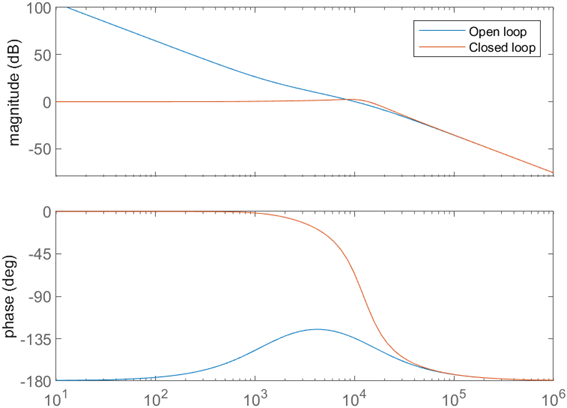
\includegraphics[width=0.7\linewidth]{Figures/Bode diagram of current control loop.png}
    \caption{Bode diagram of current control loop}
    \label{fig:bode_current}
\end{figure}

\begin{figure}[!ht]
    \centering
    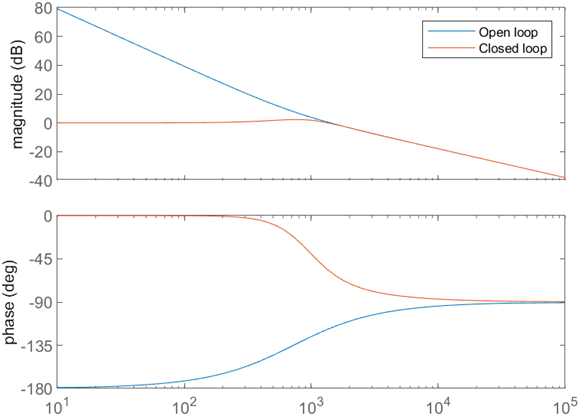
\includegraphics[width=0.7\linewidth]{Figures/Bode diagram of voltage control loop.png}
    \caption{Bode diagram of voltage control loop}
    \label{fig:bode_voltage}
\end{figure}

The cascaded PI controllers were implemented in MATLAB/Simulink and tuned further during simulation.
